% !TEX TS-program = pdflatex
% !TEX encoding = UTF-8 Unicode

% This is a simple template for a LaTeX document using the "article" class.
% See "book", "report", "letter" for other types of document.

\documentclass[11pt]{article} % use larger type; default would be 10pt 

\usepackage[utf8]{inputenc} % set input encoding (not needed with XeLaTeX)

%%% Examples of Article customizations
% These packages are optional, depending whether you want the features they provide.
% See the LaTeX Companion or other references for full information.

%%% PAGE DIMENSIONS
\usepackage{geometry} % to change the page dimensions
\geometry{a4paper} % or letterpaper (US) or a5paper or....
% \geometry{margins=2in} % for example, change the margins to 2 inches all round
% \geometry{landscape} % set up the page for landscape
%   read geometry.pdf for detailed page layout information

\usepackage{graphicx} % support the \includegraphics command and options

% \usepackage[parfill]{parskip} % Activate to begin paragraphs with an empty line rather than an indent

%%% PACKAGES
\usepackage{booktabs} % for much better looking tables
\usepackage{array} % for better arrays (eg matrices) in maths
\usepackage{paralist} % very flexible & customisable lists (eg. enumerate/itemize, etc.)
\usepackage{verbatim} % adds environment for commenting out blocks of text & for better verbatim
\usepackage{subfig} % make it possible to include more than one captioned figure/table in a single float
\usepackage{amssymb}
\usepackage{graphicx}
\usepackage{algorithmic}
\usepackage{algorithm}
\usepackage[parfill]{parskip}
\usepackage{rotfloat }
\usepackage{mathtools}
\usepackage{array}
\usepackage{tikz}
\usepackage{stmaryrd}
\usepackage{textcomp}
\usepackage{listings}
\usepackage[toc,shortcuts,nonumberlist,smallcaps,numberedsection=autolabel]{glossaries}   
\usepackage{dot2texi}
\usepackage{graphicx}

\lstset{
basicstyle=\small\sffamily,
numbers=left,
numberstyle=\tiny,
frame=tb,
columns=fullflexible,
showstringspaces=false
}

% These packages are all incorporated in the memoir class to one degree or another...


\newglossaryentry{Bohnanza}{name={Bohnanza}, description={}}
\newglossaryentry{player}{name={player}, description={}}
\newglossaryentry{field}{name={field}, description={}}
\newglossaryentry{card}{name={card}, description={}}
\newglossaryentry{treasury}{name={treasury}, description={}}
\newglossaryentry{bean}{name={bean}, description={}}
\newglossaryentry{coffee}{name={coffee}, description={}}
\newglossaryentry{wax}{name={wax}, description={}}
\newglossaryentry{blue}{name={blue}, description={}}
\newglossaryentry{chili}{name={chili}, description={}}
\newglossaryentry{stink}{name={stink}, description={}}
\newglossaryentry{green}{name={green}, description={}}
\newglossaryentry{soy}{name={soy}, description={}}
\newglossaryentry{black-eyed}{name={black-eyed}, description={}}
\newglossaryentry{red}{name={red}, description={}}
\newglossaryentry{garden}{name={garden}, description={}}
\newglossaryentry{cocoa}{name={cocoa}, description={}}
\newglossaryentry{amount}{name={amount}, description={}}
\newglossaryentry{beanometer}{name={beanometer}, description={}}
\newglossaryentry{worth}{name={worth}, description={}}
\newglossaryentry{coin}{name={coin}, description={}}
\newglossaryentry{area}{name={area}, description={}}
\newglossaryentry{bean field}{name={bean field}, description={}}
\newglossaryentry{farm}{name={farm}, description={}}
\newglossaryentry{box}{name={box}, description={}}
\newglossaryentry{oldest player}{name={oldest player}, description={}}
\newglossaryentry{hand}{name={hand}, description={}}
\newglossaryentry{draw deck}{name={draw deck}, description={}}
\newglossaryentry{discard pile}{name={discard pile}, description={}}
\newglossaryentry{dealer}{name={dealer}, description={}}
\newglossaryentry{left player}{name={left player}, description={}}
\newglossaryentry{turn}{name={turn}, description={}}
\newglossaryentry{first turn}{name={first turn}, description={}}
\newglossaryentry{second turn}{name={second turn}, description={}}
\newglossaryentry{third turn}{name={third turn}, description={}}
\newglossaryentry{fourth turn}{name={fourth turn}, description={}}
\newglossaryentry{plant}{name={plant}, description={}}
\newglossaryentry{draw}{name={draw}, description={}}
\newglossaryentry{first draw}{name={first draw}, description={}}
\newglossaryentry{last draw}{name={last draw}, description={}}
\newglossaryentry{trade}{name={trade}, description={}}
\newglossaryentry{donate}{name={donate}, description={}}
\newglossaryentry{plant hand}{name={plant hand}, description={}}
\newglossaryentry{plant traded donated}{name={plant traded donated}, description={}}
\newglossaryentry{harvest and sell}{name={harvest and sell}, description={}}
\newglossaryentry{player area}{name={player area}, description={}}
\newglossaryentry{keep area}{name={keep area}, description={}}
\newglossaryentry{draw area}{name={draw area}, description={}}
\newglossaryentry{round}{name={round}, description={}}
\newglossaryentry{round one}{name={round one}, description={}}
\newglossaryentry{round two}{name={round two}, description={}}
\newglossaryentry{round three}{name={round three}, description={}}
\newglossaryentry{shuffle}{name={shuffle}, description={}}
\newglossaryentry{buy bean field}{name={buy bean field}, description={}} 
\makeglossaries 

%%% HEADERS & FOOTERS
\usepackage{fancyhdr} % This should be set AFTER setting up the page geometry
\pagestyle{fancy} % options: empty , plain , fancy
\renewcommand{\headrulewidth}{0pt} % customise the layout...
\lhead{}\chead{}\rhead{}
\lfoot{}\cfoot{\thepage}\rfoot{}

%%% SECTION TITLE APPEARANCE
\usepackage{sectsty}
\allsectionsfont{\sffamily\mdseries\upshape} % (See the fntguide.pdf for font help)
% (This matches ConTeXt defaults)
 
%%% ToC (table of contents) APPEARANCE
\usepackage[nottoc,notlof,notlot]{tocbibind} % Put the bibliography in the ToC
\usepackage[titles,subfigure]{tocloft} % Alter the style of the Table of Contents
\renewcommand{\cftsecfont}{\rmfamily\mdseries\upshape}
\renewcommand{\cftsecpagefont}{\rmfamily\mdseries\upshape} % No bold!

%%% END Article customizations

%%% The "real" document content comes below...

\title{Patterns of Software Development \\ \small{Report on a Bohnanza Implementation}}
\author{Jeroen Meijer (s0166111)}
%\date{} % Activate to display a given date or no date (if empty),
         % otherwise the current date is printed 

\begin{document}
\maketitle
 
\section{Design goals}
The importance of particular quality criteria depend on in which environment the application is
used. This environment also influences the stakeholders; not every categorie stakeholder is affected
by the software system. We offer our system open sourced and free of charge
online.\footnote{https://github.com/Meijuh/psd}. We assume the application is a highly popular one
and is us used among many people. We identify the most important quality criteria for this
environment as \emph{extensibility} and \emph{reusability}. The most affected stakeholders are the
\emph{developers}, \emph{maintainers}, \emph{testers} and \emph{users}.

Extensibility is an external criteria; it is most important for the user. Reusability is more
important for developers etc. Both criteria are also covered under the term modularity. Modularity
allow the user to easily use one of the many extensions, such as High Bohn or spin-offs, such as Al
Cabohne. It should be easy to implement such extensions for developers etc.

There is one major design decisions that contribute to modularity. First we have three modules
which can be considered separate projects. One module contains basic objects and method related to
bohnanza, such as shuffling the discard pile into the draw deck. Another module implements \gls{std} 
bohnanza without extensions. The last module implements the \gls{hb} extension. All projects can
of course be tested and compiled individually. The \gls{std} and \gls{hb} extension inherit from the
base module. The base module provides an abstract class that resolves dependency resolution between
modules. Both the \gls{std} and the \gls{hb} module implement this class. Making it possible to hide
some information in modules and should result in understandable modules. 

\begin{itemize}
    \item Reusability
    \item Extensibility
    \item remove inadequacies
    \item adapt to changing needs
    \item extend functionality quickly
    \item integrate with other systems
    \item use components in other projects
    \item Modularity
    \item decomposability
    \item composability
    \item understandability
    \item continuity
    \item protection
    \item direct mapping
    \item few interfaces
    \item small interfaces
    \item explicit interfaces
    \item information hiding
    \item 
\end{itemize}

\section{Design}

Our design is split up in three modules.
\begin{description}
    \item[bohnanza] {Mostly an abstract base module that contains logic for both the \gls{std} and
    \gls{hb} game.}
    \item[bohnanza-std] {A concrete module that uses the \emph{bohnanza} module in order to play
    the \gls{std} bohnanza game.}
    \item[bohnanza-hb] {A concrete module that uses the \emph{bohnanza} module in order to play the
    \gls{hb} bohnanza game.}
\end{description}
The reason why these elements are composed this way and called modules is a result of the dependency
injection (Guice\footnote{https://code.google.com/p/google-guice/}) framework we use. This framework supplies abstract module classes which
need to be implemented. Such a module class contains a set of dependencies. For example the bohnanza module uses an abstract Player class.
Both the bohnanza-std and bohnanza-hb module use an concrete implementation hereof. Another reason why these modules are composed this way
is due to the fact that we chose that an extension (and the \gls{std} game) should extend classes of the base game and not implement hooks. 

Every module is designed according to the MVC pattern. The main classes that are involved in the MVC pattern are shown in Figure
\ref{fig:design:mvc}.

 \begin{figure}[h!]
    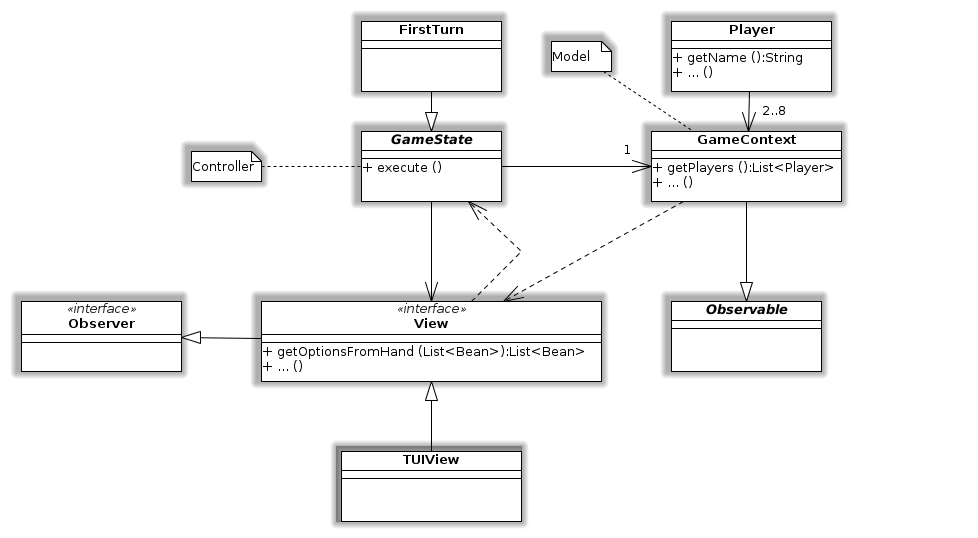
\includegraphics[width=\textwidth]{../img/Mvc}
    \caption{Classes involved in MVC}
    \label{fig:design:mvc}
\end{figure}

The \texttt{GameContext} is the main model class. It contains many assocations to other model classes such as the \texttt{Player}. Many
model classes are \texttt{Observable} by \texttt{Observer}s such as the \texttt{View} class. This is how the view knows the status of the
model. The \texttt{GameState} is the controller which updates the view and the model. The controller issues method calls such as
\texttt{getOptionsFromHand()} which returns a sub set of \texttt{Bean} cards. The controller is part of a \emph{state} pattern. An
alternative to the MVC pattern is the Model View Presenter pattern which could have been applied in this context. We chose to keep things
simple and focus more on the extensibility of bohnanza rather than on implementing other views such as a graphical one. We think that the
classic MVC pattern suffices here.
 
\subsection{Model}
Three important parts of the model involve the hierarchy of cards (Figure \ref{fig:design:cards}),
the creation of cards (Figure \ref{fig:design:creator}) using a \emph{factory method} pattern and
the relation between different sets of cards and the players (Figure \ref{fig:design:player}). 

 \begin{figure}[h!]
    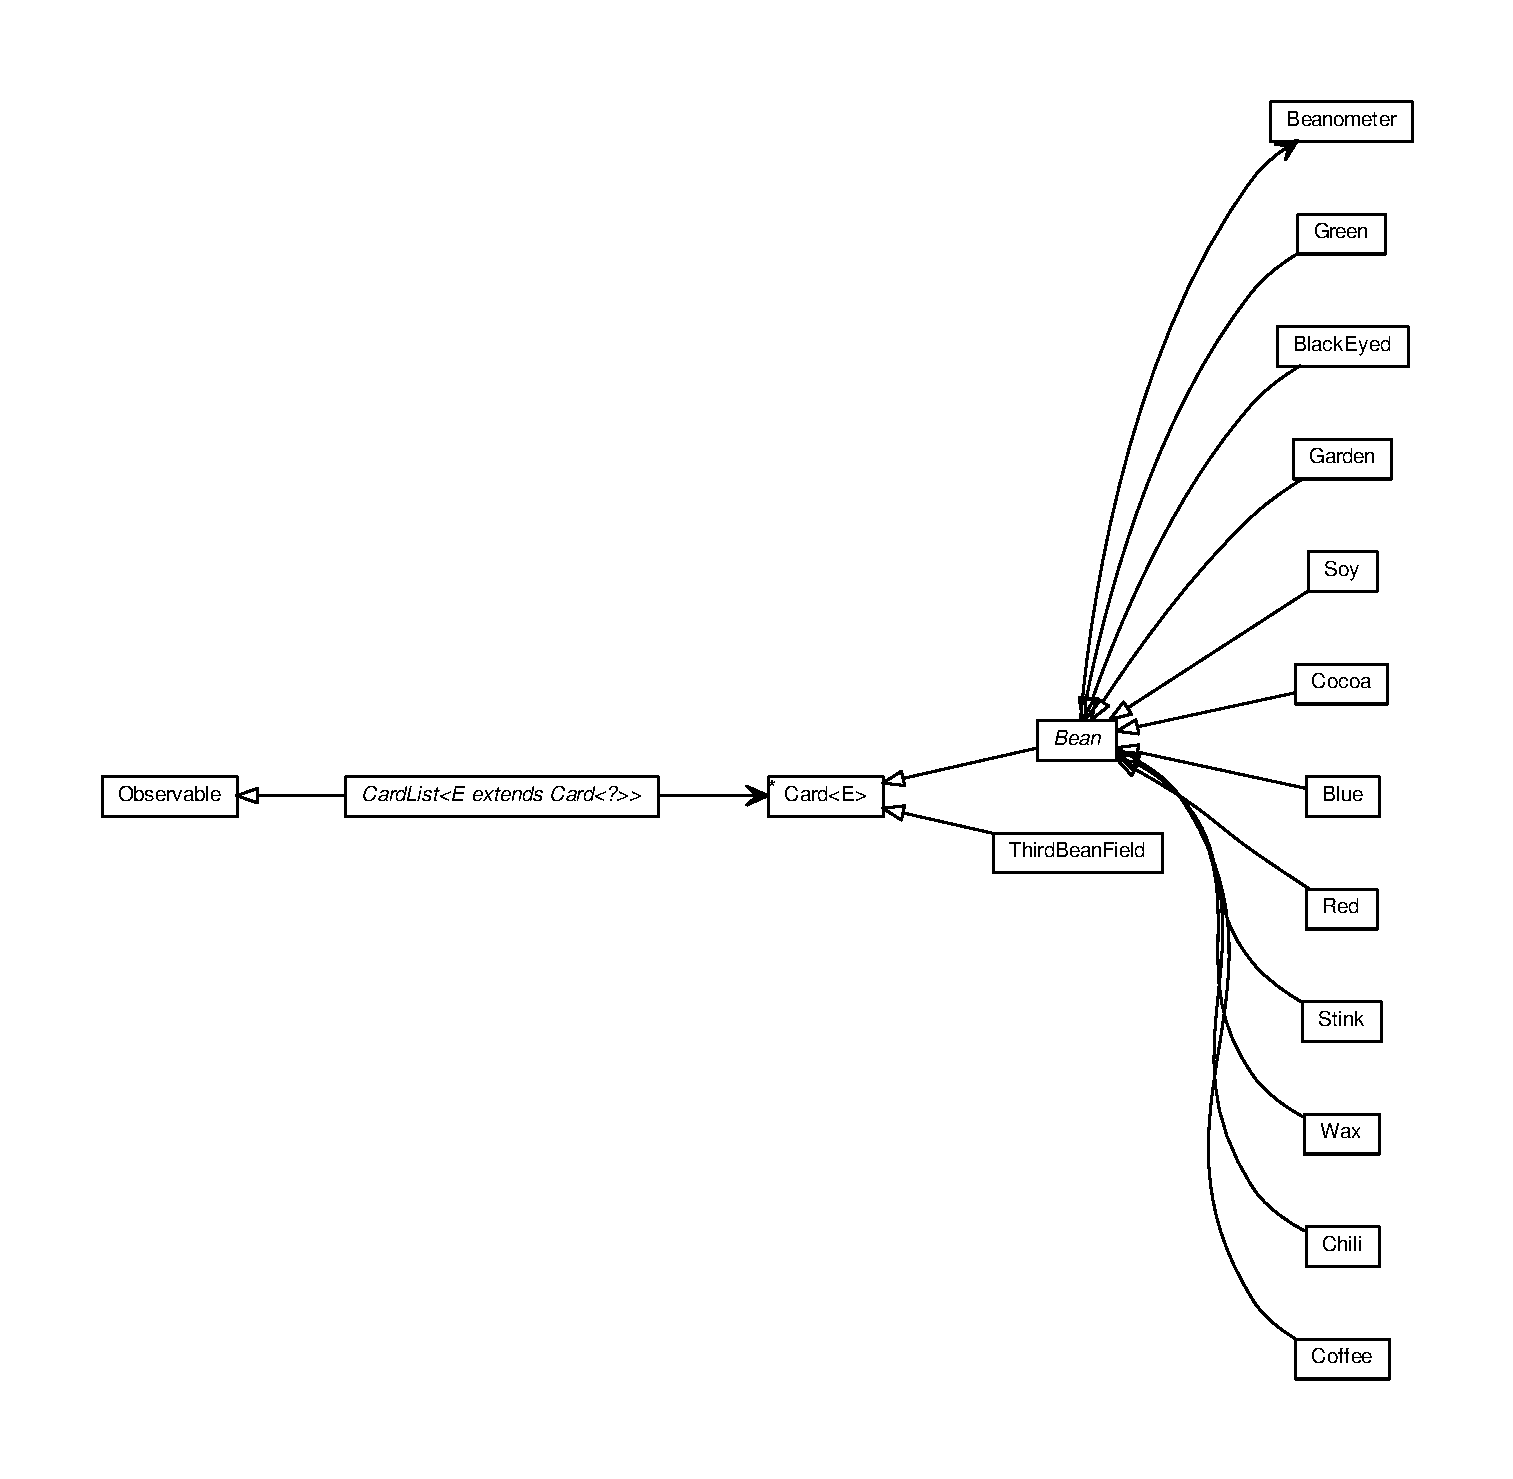
\includegraphics[width=\textwidth]{../umlgraph/CardGraph}
    \caption{Class diagram of the cards}
    \label{fig:design:cards}
\end{figure}

\begin{figure}[h!]
    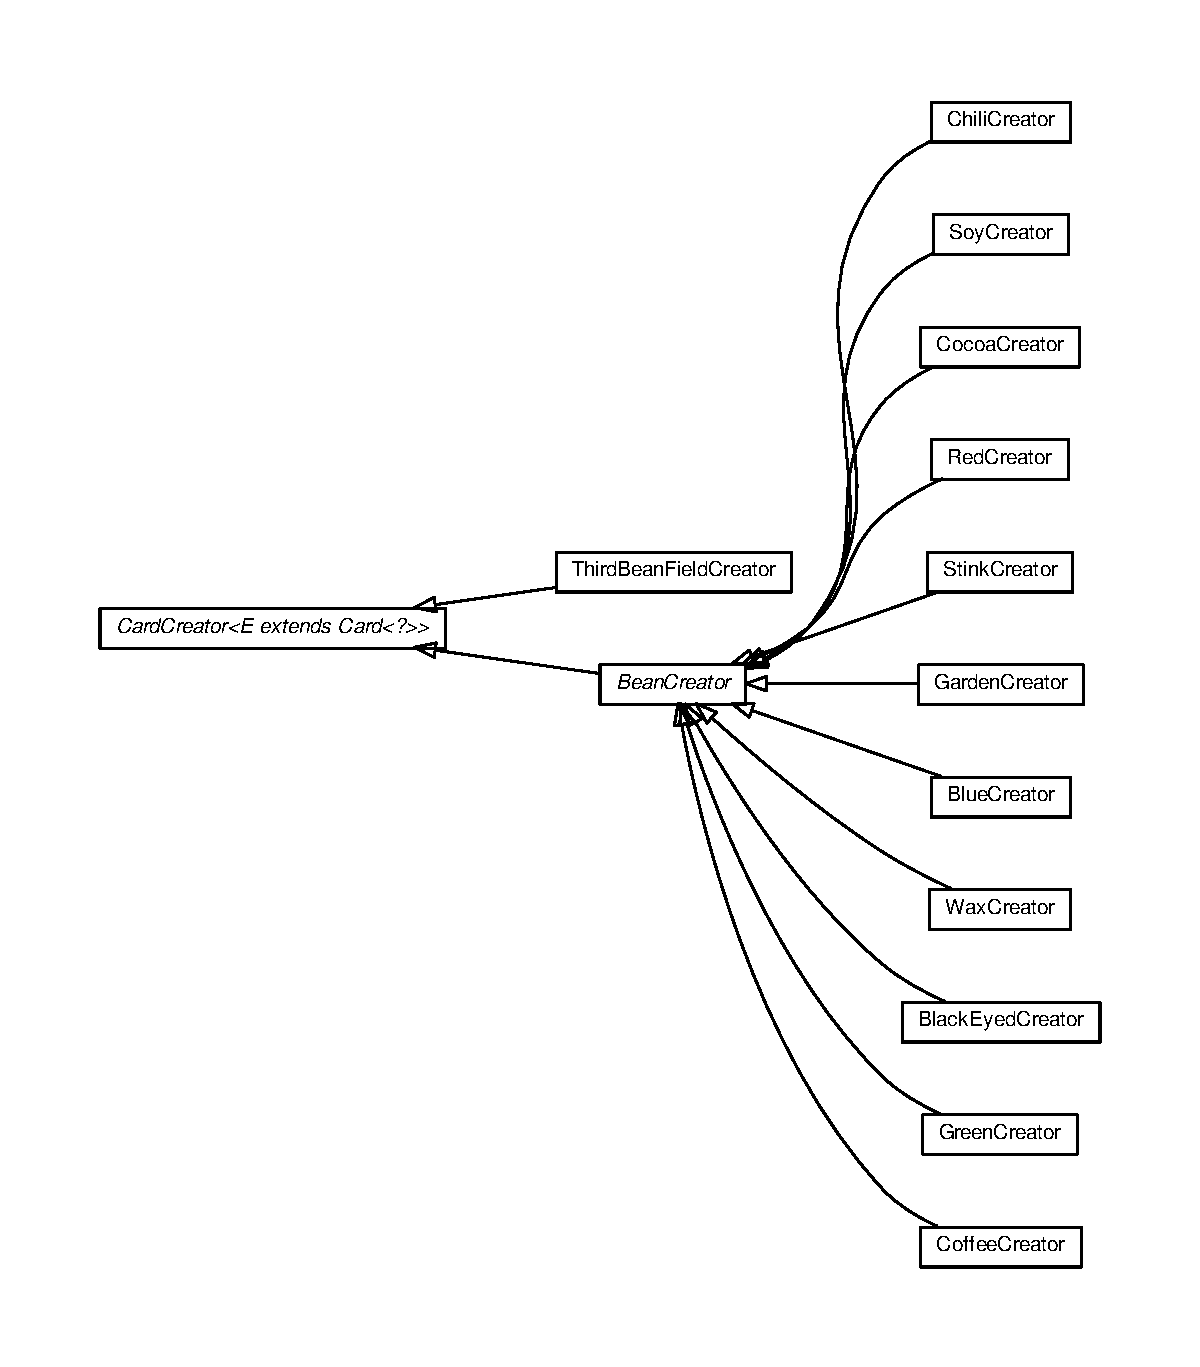
\includegraphics[width=\textwidth]{../umlgraph/CreatorGraph}
    \caption{Class diagram for the creation of cards}
    \label{fig:design:creator}
\end{figure}

The hierarchy of the cards here is convenient, namely when creating extensions of bohnanza. When new cards are introduced to the game
creating a new factory i.e. subtyping \texttt{CardCreator} or \texttt{BeanCreator} is easy because those factories expect a subtype of a
\texttt{Card}. Instead of using a factory method pattern we could have approach this a little different. Guice allows creating multiple
instances of a class by means of a \texttt{Provider} class. Using this alternative would have resulted in cleaner code. The reason why we
did not choose this alternative is because we introduced Guice into our project after we used the factory method pattern and did not want to
rewrite our code. We did however use the provider method for creating \texttt{Player}s as shown in Figure \ref{fig:design:di}, because this
was the only way to inject these objects into an \texttt{Bohnanza} object.

\begin{figure}[h!] 
    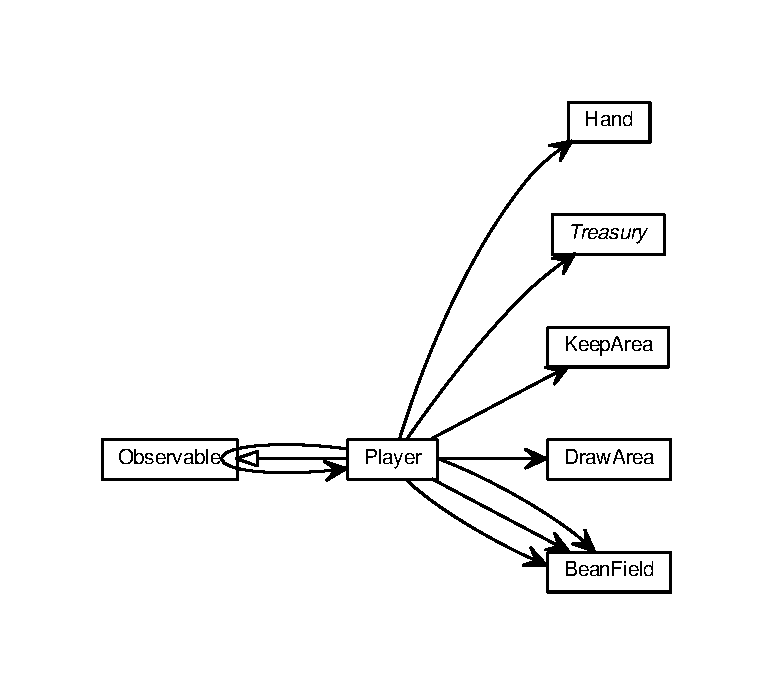
\includegraphics[width=\textwidth]{../umlgraph/PlayerGraph}
    \caption{Class diagram for the player and association to particular sets of cards}
    \label{fig:design:player}
\end{figure}

\newpage
\subsection{Controller}
The controller of the game is implemented using a \emph{state} design pattern and is shown in Figure
\ref{fig:design:controller}. An alternative we could use here is the \emph{strategy} pattern. The strategy pattern is more applicable in
situations where strategies are chosen at runtime. But more importantly the strategy pattern is used in situation where the result of
different strategies is the same. In bohnanza the order of states is rather fixed the order only varies depending on how often the deck is
shuffled or in case of execeptional behaviour. In case exceptional behaviour occurs in our application the next state is always the
\texttt{Fail} state. In general the order of states that are executed are \texttt{Prepare} \textrightarrow{} \texttt{FirstTurn}
\textrightarrow{} \texttt{SecondTurn} \textrightarrow{} \texttt{ThirdTurn} \textrightarrow{} \texttt{FourthTurn} \textrightarrow{}
\texttt{FirstTurn} \textrightarrow{} \ldots \textrightarrow{} \texttt{End}. A typical implementation of the \texttt{GameState.execute}
method is shown as follows in \texttt{FirstTurn}. Note how the next state is set by getting the singleton instance on Line 19. The
application continues until a \texttt{GameState} sets the next state to \texttt{null}, i.e. when \texttt{GameContext.getState() == null}.

\begin{lstlisting}[language=Java, caption=FirstTurn.execute()]
@Override
public void execute(GameContext context) {

    if (context.getCurrentPlayer().getHand().size() > 0) {

        int beanFieldNumber = context.getView().mustPlant(context.getCurrentPlayer());

        try {

            context.getCurrentPlayer().plantHand(beanFieldNumber);
 
            if (context.getCurrentPlayer().getHand().size() > 0) {
                beanFieldNumber = context.getView().mayPlant(context.getCurrentPlayer());

                context.getCurrentPlayer().plantHand(beanFieldNumber);

            }

            context.changeState(SecondTurn.getInstance());

        } catch (BohnanzaException e) {
            context.changeState(Fail.getInstance());
            Fail.getInstance().setException(e);
        }
    }
}
\end{lstlisting}

\begin{figure}[h!]
    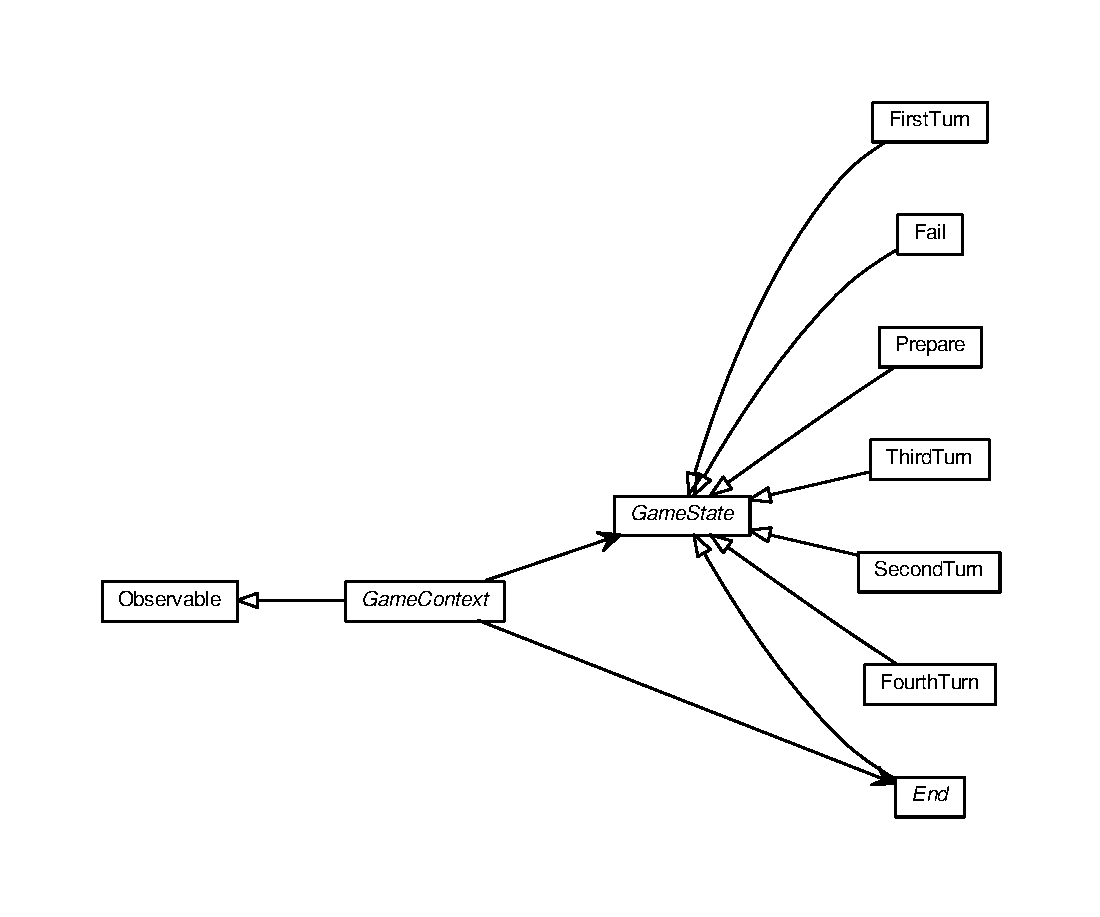
\includegraphics[width=\textwidth]{../umlgraph/StateGraph}
    \caption{Class diagram for controlling the state of the game}
    \label{fig:design:controller}
\end{figure}

\subsection{View}
Currently we support only a textual user interface. The \texttt{TUIView} class is an implementation
of a \texttt{View} interface. Creating a new interface like a graphical or a network would involve
implementing the \texttt{View} interface.

\subsection{Packages}
Our modules contain the following packages.
\begin{description}
\item[bohnanza] contains the main class.
\item[bohnanza.game] contain some models for bohnanza, such as a \texttt{Card}.
\item[bohnanza.game.factory] contains classes w.r.t. the creation of cards.
\item[bohnanza.game.player] contains model classes w.r.t. the player.
\item[bohnanza.game.shared] contains model classes which may be accessed by all players.
\item[bohnanza.game.gameplay] contains controller classes w.r.t. the discussed state pattern.
\item[bohnanza.module] contains classes w.r.t. dependency injection of Guice.
\item[bohnanza.umlgraph] contains classes that model UML graphs used in this report.
\item[bohnanza.view] contains the view classes.
\end{description}

The packages are rather self explainatory. It can be argued however that some packages such as \texttt{bohnanza.game.player} and
\texttt{bohnanza.game.shared} may be merged. In an early stage of the development we chose to make some classes \emph{package private} such
that for example only a \texttt{Player} could construct a \texttt{Hand} this would make sure there can only be as many \texttt{Hand}s in the
game as there are \texttt{Player}s. This design choice was one of the reasons our code was not testable and we had to change the visibility
parameters to use dependency injection.

\subsection{Variations}

\subsubsection{User}
The user can specify during the startup of the application how many players there are using a
commandline option. For example \texttt{java bohnanza.BohnanzaStd -p=3} starts the BohnanzaStd
module with three players. Parsing commandline options is done using the Apache Commons CLI library.

\subsubsection{Developer}
Variability for the develop depends heavily on notion of \emph{dependency injection}. Dependency
injection is a design pattern that basically involves moving dependency resolution from a particular
class to a framework dedicated to dependeny injection. We use Guice for this. Classes involved with dependency injection are shown in
Figure \ref{fig:design:di}. If a developer wants another variation of the application the developer can simply extend the
\texttt{BohnanzaModule} class and define other classes to inject, note that BohnanzaModule
extends the \texttt{AbstractModule} class from Guice. For example if a \texttt{Hand} object needs
to behave differently for a particular extension of bohnanza one can extend Hand and
define the extension in the extension of BohnanzaModule. BohnanzaModule itself is
an abstract class and this class only knows the full list of required dependencies. A concrete class
such as BohnanzaStdModule implements some methods that return concrete classes as
dependencies. This relates closely to the \emph{single choice principle}. Listing \ref{lst:di} shows how one can change dependencies using
an extension of the AbstractModule class. Note how the singleton pattern and the provider incoorporate nicely in the configure method.

\begin{lstlisting}[language=Java, caption=BohnanzaModule.java, label=lst:di]
public abstract class BohnanzaModule extends AbstractModule {

    @Override
    protected void configure() {
        bind(View.class).to(getViewClass());
        bind(DrawDeck.class).in(Singleton.class);
        bind(Player.class).toProvider(getPlayerProviderClass());
        ...
    }

    protected abstract Class<? extends Provider<? extends Player>> getPlayerProviderClass();
    protected abstract Class<? extends DrawDeck> getDrawDeckClass();
    protected abstract Class<? extends View> getViewClass();    
    ...
}
\end{lstlisting}

We have not really considered an alternative to dependency injection, because to our knowledge there is no real alternative
for it. There is however the service locater pattern, but both these patterns solve a problem which
is not that hard, that is injecting instances of some classes in another object instead of
constructing these instances in that particular object. We found that Guice was a good enough
framework, so we did not consider an alternate framework.

\begin{figure}[h!]
    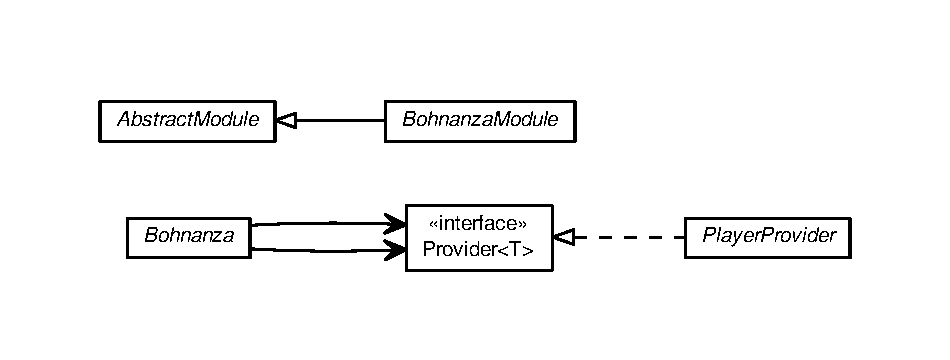
\includegraphics[width=\textwidth]{../umlgraph/ModuleGraph}
    \caption{Class diagram of classes involving dependency injection}
    \label{fig:design:di}
\end{figure}
  
\section{testing}
\begin{itemize}
\item{The main goal of our testing approach is to test the more complex parts of game such as
trading. One of our goals is not to achieve 100 percent test coverage, but to test the complex parts
in a a nice way. }
    \item {
Our design is wel suited for testing. Since our design adheres to the dependency injection pattern
injecting mocked objects of classes is easy. For mocking we used the
Mockito\footnote{https://code.google.com/p/mockito/} framework.}
\item {Each of the three modules can be compiled and tested separately. However the \emph{bohnanza}
module is rather abstract and thus testing some abstract classes do not really make sense. We test
more concrete classes in either the \gls{std} module or the \gls{hb} module.}
\item {In the bohanza module we mainly tested whether the \texttt{Beanometer} or \texttt{CardList}
works correctly. This is shown in the coverage report in the package \texttt{bohnanza.game}. Since a
game can not really be played in the bohnanza module the gameplay is tested in a concrete
implementation of bohnanza, namely bohnanza-std. This is shown in the package
\texttt{bohnanza.gameplay}}.
\end{itemize}

\begin{figure}[h!]
    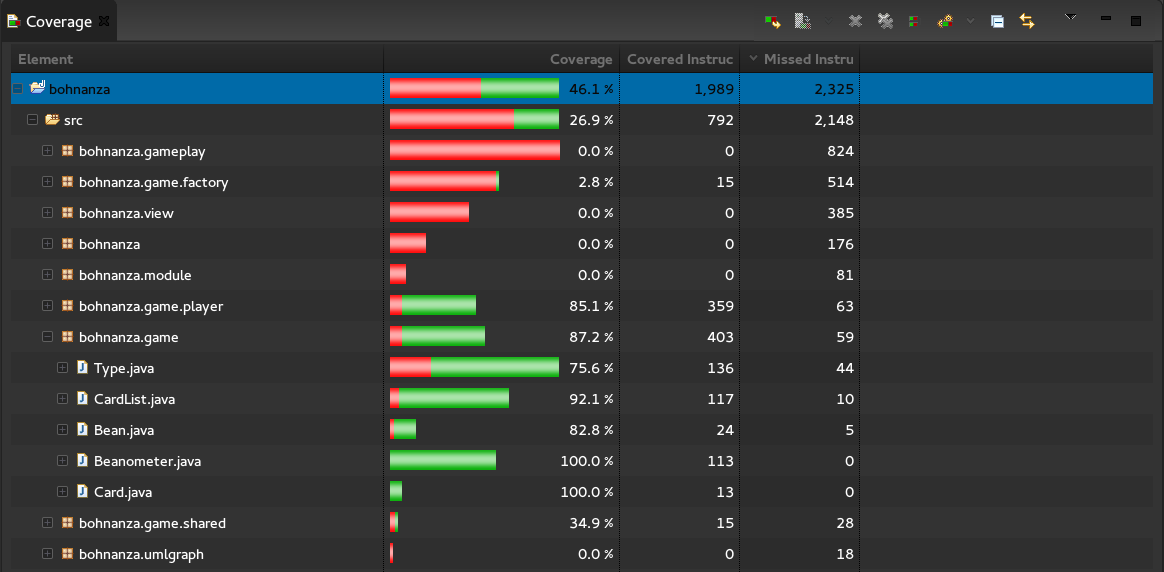
\includegraphics[width=\textwidth]{../img/coverage}
    \caption{Coverage of the \emph{bohnanza} module}
    \label{fig:test:coverage}
\end{figure}

\begin{figure}[h!]
    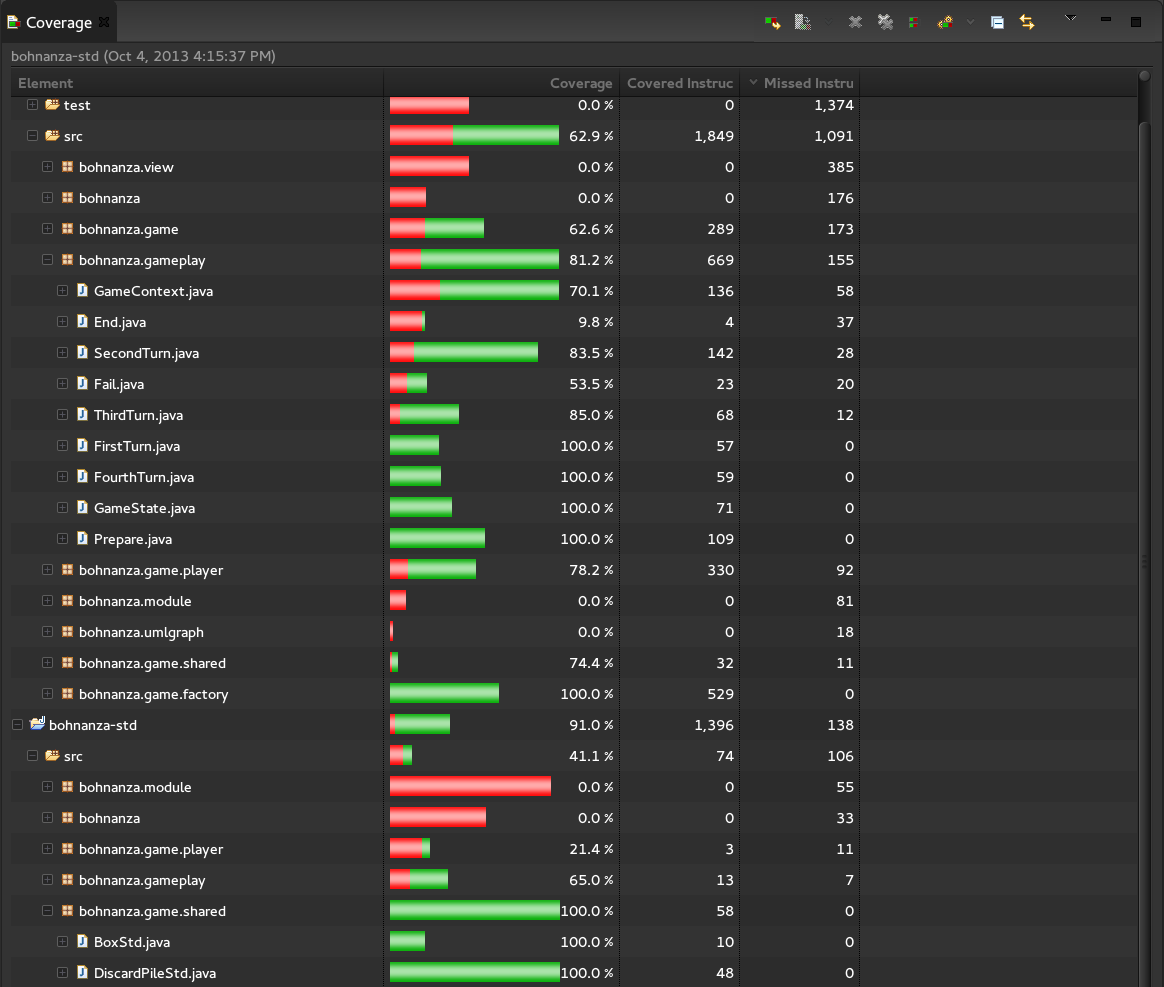
\includegraphics[width=\textwidth]{../img/coverage-std}
    \caption{Coverage of the \emph{bohanza-std} module}
    \label{fig:test:coverage-std}
\end{figure}
 
\section{development process}
First we drew a class diagram using Software Ideas Modeler\footnote{http://www.softwareideas.net/} including methods and attributes. Using
this diagram we generated Java class skeletons. Soon we came to the conclusion that many parts of our application could not be
tested well, because we tried to protect it from incorrect behaviour to much by minimizing the amount of collaborations.

% This involved creating specific instances of classes in
% constructors and hiding away to much by creating wrapper classes. One example of such a wrapper class is a \texttt{PlayerArea} which
% contains the beanfields, hand, etc, but not the discard pile. The idea is that we could use such a wrapper class to make sure some
% operations could not be done, such as moving a card from a hand to the discard pile. We did not use this approach because it was not
% testable. We removed the wrapper classes and used a dependency injection framework instead.

After standard bohnanza was implemented we began working on high bohn. We decided we could use the dependency injection framework to create
the three modules. At this moment in time we saw that in order to have both the standard and high bohn implementation we needed three
instead of two modules. The main reason is that you should design for extension as suggested by Checkstyle (see subsection
\ref{ssec:flexibility}). 
% This means one should
% explicitly make some methods abstract which should be implemented by a more concrete class. Our first intention was to just override some
% methods which needed different behaviour in high bohn than that in standard bohnanza.

After we were done with the implementations we used
UmlGraph \footnote{http://www.umlgraph.org/doc/indexw.html} to generate necessary class diagrams and write this report. 

Our design phase was rather short; we drew only a class diagram. In a bachelor course we learned proper software design with several phases
such as domain analysis, domain models, high level designs, detailed designs and more. The class diagram we drew for bohnanza is most
reasonably a detailed design. We find that the method learned during the bachelor course is well suited for creating complex software systems,
but since this approach does not fit well in the required report for this assignment (it should focus on the detailed design) we decided to
focus more on explaining design decisions and applied techniques.
 
\section{lessons learned}
Only rather late in the development process we came to the conclusion that our implementation was hard to test. Should we have used a Test
Driven Development we would have come to the conclusion to use dependency injection much earlier. So on the principle of making testable
code we might have failed, but we learned. Now we know that dependency injection is key to making testable code we do not think TDD is key
we find that sometimes implementing first and then generate a unit test to some degree can be just as convenient.

Some good principle we have learned came from using tools. After we installed moreunit it suggested to use the Mockito framework. This
allowed us to easily mock classes such as the view. Instead of subtyping a view class we could simply invoke \texttt{View view =
mock(View.class);} and \texttt{when(view.getOptionsFromHand())} \\ \texttt{.thenReturn(new ArrayList<Bean>());}. But more importantly what
we learned is that one should not do partial mocking. That is either one should mocking everything of a class or nothing. Partial mocking is
done by mocking one method and invoke the real implementation of an other method. Mockito warns the developer when he/she uses partial
mocking. Since mocking does not allow assigning values to private fields of mocked objects one has to \emph{verify} behaviour. In Mockito
this can be done with the \texttt{verify} method, e.g. \texttt{verify(discardPile, atLeastOnce()).add(new BlackEyed());}. For verifying
advanced argument captors can be used and asserting that such a captor contains a certain value.

Another good principle we have learned came from using Checkstyle. Checkstyle warned us about the fact that a method should either be final
or abstract, which we discussed earlier.

Furthermore we have learned there is only one good free and open source tool for generating class diagrams. This tool is called UMLGraph and
uses Java classes for specifying -- with visibility parameters -- certain \emph{view}s on your design. To generate these diagrams one has to
pass a custom doclet to the javadoc command. Visual Paradigm \footnote{http://www.visual-paradigm.com/} is a closed source and costly
alternative which also supports round-tripping which is very convenient for larger projects.

\glsaddall
\glossarystyle{superheader} 
\printglossaries

% \section{appendix}





% \bibliographystyle{plain} 
% \bibliography{references} 

\end{document}